“Aviso! Não cometa o erro de assumir que a agilidade lhe dará licença para abreviar soluções. Processo é um requisito e disciplina é essencial” \cite {pressman}

Segundo Pressman, para projetos que adotam uma filosofia de desenvolvimento de software ágil, um ambiente ideal seria aquele em que engenheiros de software trabalham juntos na mesma equipe.

Visto que a abordagem ágil requer uma proximidade com o cliente, o grupo chegou a conclusão que a tal abordagem poderia vir a se adequar melhor ao contexto de negócio, visto que a diretora da empresa cliente possui disponibilidade de tempo para fazer reuniões semanais com a equipe, e ainda por a empresa ser sediada na Universidade de Brasília, campus Gama, local onde se encontra os Analistas de Requisitos da equipe.

Outro fator determinante foi o notório conhecimento, ainda que básico, demonstrado pela diretora da Eletrojun em um primeiro contato com a mesma, de forma a corroborar para a decisão de metodologia a ser adotada. Esta relatou já ter participado efetivamente de processos de requisitos, orientando desenvolvedores da própria empresa, demonstrando aptidão para fases de elicitação e acompanhamento de requisitos em processo ágil.

Quanto aos modelos de maturidade, optou-se pelo modelo MPS-BR. Este modelo apresenta vantagens em relação ao ao modelo CMMI entre as quais destacam-se:

\begin{itemize}
\item MPS-BR é um modelo nacional, se enquadrando melhor a realidade brasileira.
\item É um modelo pautado em pequenas e médias empresas, então se encaixa. perfeitamente ao contexto presente.
\item Financeiramente, o MPS é mais barato e se enquadra melhor no contexto da empresa, visto que o modelo CMMI possui um custo consideravelmente mais elevado.
\item O projeto possui não possui uma extensão internacional.
\end{itemize}

\section {Panorama Ágil}

O manifesto foi feito em 2001 por 17 desenvolvedores que foram na contramão da produção de software tradicional. O manifesto passava a valorizar os indivíduos e interações mais que os processos e ferramentas, o software funcionando mais que a documentação abrangente, colaboração do cliente mais que negociação de contrato, e responder a mudanças mais que seguir um determinado plano.

O manifesto ágil surge com o intuito de sanar as fraquezas  reais e perceptíveis da maneira tradicional de produção de software. Apesar da metodologia fornecer benefícios importantes, não é indicada em todas as situações, porque “There is no silver bullet” (Fred Brooks) não existe a bala de prata para a metodologia de desenvolvimento empregada no projeto, tudo vai ter que ser analisado para que se chegue a metodologia mais sensata ao projeto.

\section{Alterações e mudanças no ágil}

Atualmente na economia é difícil prever como uma aplicação irá evoluir em acordo com o tempo devido as condições de mercado. O mercado muda com uma frequência muito difícil de prever, regras de negócio e as necessidades dos usuários finais são as áreas mais afetadas, além disso novas ameaças competitivas surgem inesperadamente no mercado. Em muitas dessas situações não será possível definir completamente os requisitos antes de iniciar o projeto para adaptar-se a competitividade do mercado.

As mudanças no projeto quando não planejadas implicam em custos elevados. Uma das grandes vantagens do ágil é sua adaptabilidade a mudança, reduzindo os custos ao longo de todo o processo de software.

\FloatBarrier
\begin{figure}[!htpd]
		\centering
		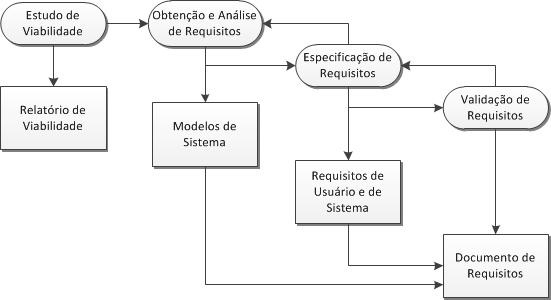
\includegraphics[scale=1.0]{figuras/processo_ER}
		\label{img:SAF}
		\caption{Processo geral de Engenharia de Requisitos}
\end{figure}
\FloatBarrier

\section{Desenvolvimento Ágil x RUP}

Hoje em dia ainda existe o mito de que a metodologia ágil é a bala de prata para o processo de desenvolvimento, e que o método tradicional acaba por atrasar, enrolar, ou gerar um trabalho inútil com uma documentação que não serve para nada. O que é comprovado atualmente é que independente da abordagem, ou se são usadas as práticas do PMBOK.
Atualmente grande partes das empresas andam adotando modelos híbridos, adaptando principalmente metodologias tradicionais ao contexto do projeto. Uma das grades reclamações sobre o IRUP – IBM Rational Unified process, da IBM, é a grande quantidade de artefatos gerados, sendo que a única coisa que é preconizada no IRUP são as 4 fases do processo, iniciação, construção, elaboração e transição. Uma das primeiras frases do livro IRUP fala que o processo deve ser customizado em acordo com as necessidades das organizações \cite {rup}.

“The Rational Unified Process is a configurable process. No single process is suitable for all software development.”

Resumidamente é dito que o processo é reconfigurável, que não existe um único processo que seja adequado para todo desenvolvimento de software.

A metodologia ágil ainda é interpretada erroneamente como uma metodologia que tudo de pode, exemplificando melhor, podemos desenvolver sem documentação e sem nenhum padrão de projeto. Essa interpretação é totalmente errônea, tendo em vista que grades empresas, tanto do setor de produção software quanto de outros setores industriais usam ágil e mantêm um nível de organização de projeto e documentação excelente.

Pressman cita em seus livros que uma das prioridades do ágil é a entrega do produto, mas em meio a tantos dizeres sobre ágil, Ivar Jacobson diz que ser ágil virou moda, e explica o que é ágil na sua concepção:

“Uma equipe ágil é aquela rápida e capaz de responder apropriadamente a mudanças. Mudanças têm muito a ver com desenvolvimento de software. Mudanças no software que está sendo criado, mudanças nos membros da equipe, mudanças devido a novas tecnologias, mudanças de todos os tipos que poderão ter um impacto no produto que está em construção ou no projeto que cria o produto.”

Já é mais que comprovado que o ágil é a metodologia de desenvolvimento de software que melhor se adapta a mudanças. O suporte para mudanças no ágil é incorporado em tudo que é desenvolvido, tratado pelo próprio Ivar Jacobson como o coração e a alma do software.
